\documentclass[10pt]{article}

% usepackage serve para incluir pacotes, 
% os abaixo s�o fundamentais para permitir o uso de acentos
\usepackage[portuguese]{babel}
\usepackage[latin1]{inputenc}
% essa linha inclui um pacote que permite adicionar figuras
\usepackage[dvips]{graphicx}

\title{Exemplo Latex}
\author{Mozart Lemos de Siqueira}
\date{}

\begin{document}
%\pagestyle{empty}    %sem numera��o de pg
\maketitle
%***************************************************************Introducao
\section{Introdu��o}

%*************************************************************************
\section{Estado da Arte}

\begin{figure}[!h]
\centering
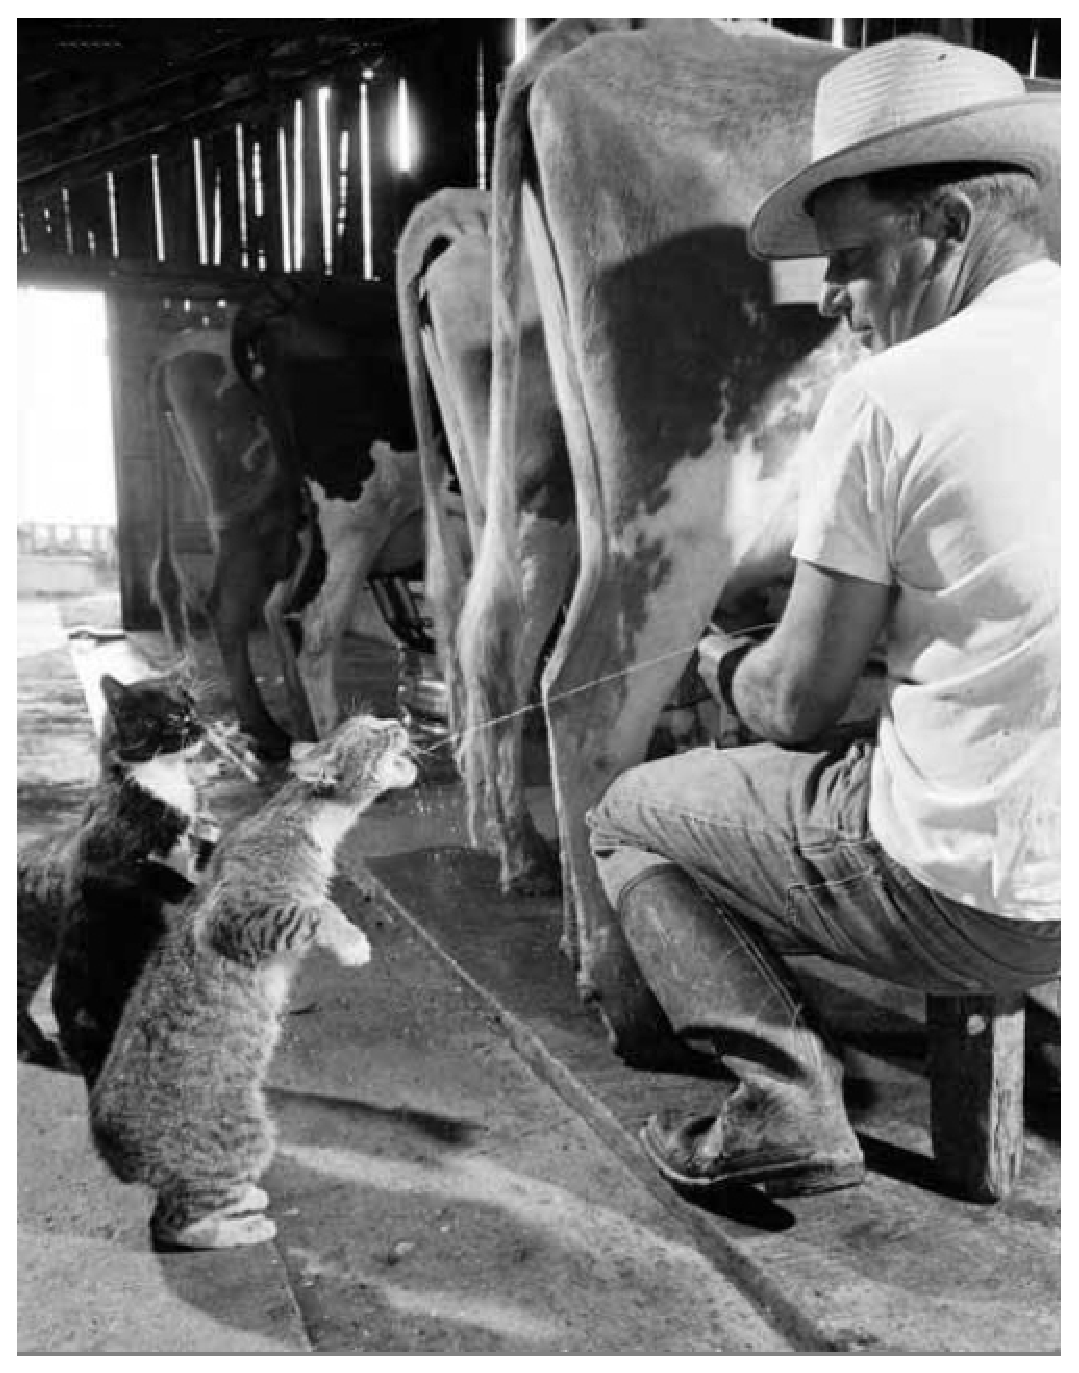
\includegraphics[width=0.5\textwidth]{leite.eps}
\caption{Exemplo de Figura}
\label{fig:ex}
\end{figure}

%*************************************************************************
\section{Metodo Proposto}
Na figura \ref{fig:ex} podemos analisar um exemplo de inser��o!

%*************************************************************************
\section{Reseultado}
Exemplo de inclus�o de refer�ncia e bibliografia \cite{Son2000}!
%*************************************************************************
\section{Conclus�o}

%*************************************************************************
%\bibliographystyle{sbc}
\bibliographystyle{plain}

\bibliography{biblio-ex}


\end{document}
